\documentclass[fleqn,usenatbib]{mnras}
%
%\hypersetup{draft}  %%% only for draft

%\usepackage{natbib}
\usepackage{xr-hyper}

%from mnras:
\usepackage{hyperref}	% Hyperlinks
\hypersetup{colorlinks=true,linkcolor=blue,citecolor=blue,filecolor=blue,urlcolor=blue}

\usepackage[russian]{babel}
\usepackage[utf8]{inputenc}

\usepackage{mathptmx}
\usepackage[T1]{fontenc}
\usepackage{ae,aecompl}
\usepackage{graphicx}	% Including figure files
\usepackage{amsmath}	% Advanced maths commands
\usepackage{amssymb}	% Extra maths symbols
\usepackage{multicol}   % Multi-column entries in tables
\usepackage{bm}         % Bold maths symbols, including upright Greek
\usepackage{pdflscape}  % Landscape pages
\usepackage{enumitem}
\usepackage{xspace}
\usepackage{hhline}
\def\beq#1{\begin{equation}\label{#1}}
\def\eeq{\end{equation}}

\usepackage{comment}

\usepackage{color}
\newcommand{\red}[1]{\textcolor{red}{#1}}
\newcommand{\blue}[1]{\textcolor{blue}{#1}}
\newcommand{\green}[1]{\textcolor{green}{#1}}
\newcommand{\achtung}[1]{\textcolor{red}{//#1//}}


\title[ShortTitle]{Title}
\author[Borisov et al.]{Victor Borisov, Alexander Meshcheryakov %\newauthor 
}
\date{September 2020}

%%%%%%%%%%%%%%%%%%%%
%DO NOT CHANGE
\makeatletter
\newcommand*{\addFileDependency}[1]{% argument=file name and extension
  \typeout{(#1)}
  \@addtofilelist{#1}
  \IfFileExists{#1}{}{\typeout{No file #1.}}
}
\makeatother

\newcommand*{\myexternaldocument}[1]{%
    \externaldocument{#1}%
    \addFileDependency{#1.tex}%
    \addFileDependency{#1.aux}%
}
%%%%%%%%%%%%%%%%%%%%
%CHANGE
%\myexternaldocument{pdf_figures}
%%%%%%%%%%%%%%%%%%%

\begin{document}
\maketitle
\begin{abstract}
Проведено исследование, построение и сравнение моделей вероятностных прогнозов фотометрических красных смещений (photo-z) на основе алгоритма случайного леса  с использованием данных современных астрономических обзоров SDSS, PanStarrs и DESI Legacy Survey для построения трехмерной карты квазаров.

Предложена модель photo-z, значительно превосходящая (в ~2 раза) по точности (метрики точечных прогнозов — нормализованное медианное абсолютное отклонение NMAD и доля выбросов n>0.15) лучшие модели (SOTA) известные в литературе. Для рентгеновских источников в тестовой области неба Stripe82X получена точность NMAD = 0.034 / 0.064 / 0.067 и n>0.15 = 0.079 / 0.170 / 0.163 для предложенной модели / шаблонной модели Ananna, 2017 / нейросетевой модели Brescia, 2019, соответственно.
\end{abstract}

% \section{Introduction}\label{sec:intro}
% \section{Related work}\label{sec:related_work}

% \section{Data}\label{sec:data}

% \section{Models}\label{sec:algos}

% \section{Metrics}

% \section{Results}\label{sec:exps}

% \begin{table*}
	\begin{tabular}{llll}
            \hline
                                           Model &          $NMAD$ &        $n>0.15$ & $n(dz_{norm}>0.15 | zConf<0.4)$ \\
            \hline
             SDSS + Pan-STARRS + DESI LIS + WISE &  \textbf{0.029} &  \textbf{0.088} &                           0.185 \\
                    Pan-STARRS + DESI LIS + WISE &           0.031 &            0.09 &                           0.177 \\
                               Pan-STARRS + WISE &           0.037 &           0.094 &                  \textbf{0.159} \\
                                 DESI LIS + WISE &            0.05 &           0.115 &                           0.353 \\
            \hline
            \end{tabular}
            \caption{Objects of Stripe82x-A17 sample sample with spec-z < 0.5 (602 objects)}
\end{table*}
% \section{Conclusions}\label{sec:results}

% \section{Discussion}\label{sec:discussion}


\section{Inctoduction}


\section{Data}
\subsection{Photometric data}
\subsection{Account for extinction}
\subsection{Train sample}
\subsection{Stripe82X test sample}
\subsection{Test sample of DR16q objects}


\section{The algorithm}
\subsection{Random forest}
\subsection{Random forest adoptation for probabilistic predictions}
\subsection{Features sets}


\section{Metrics}
\subsection{Point-estimates metrics}
\subsection{Confidence intervals metrics}
\subsection{Distribution metrics}


\section{Results}
\subsection{Optical Quasars}
We test our models in two ways: 2-fold cross-validation and quasars of SDSS DR16q.

\begin{figure*}[ht]
    \centering
    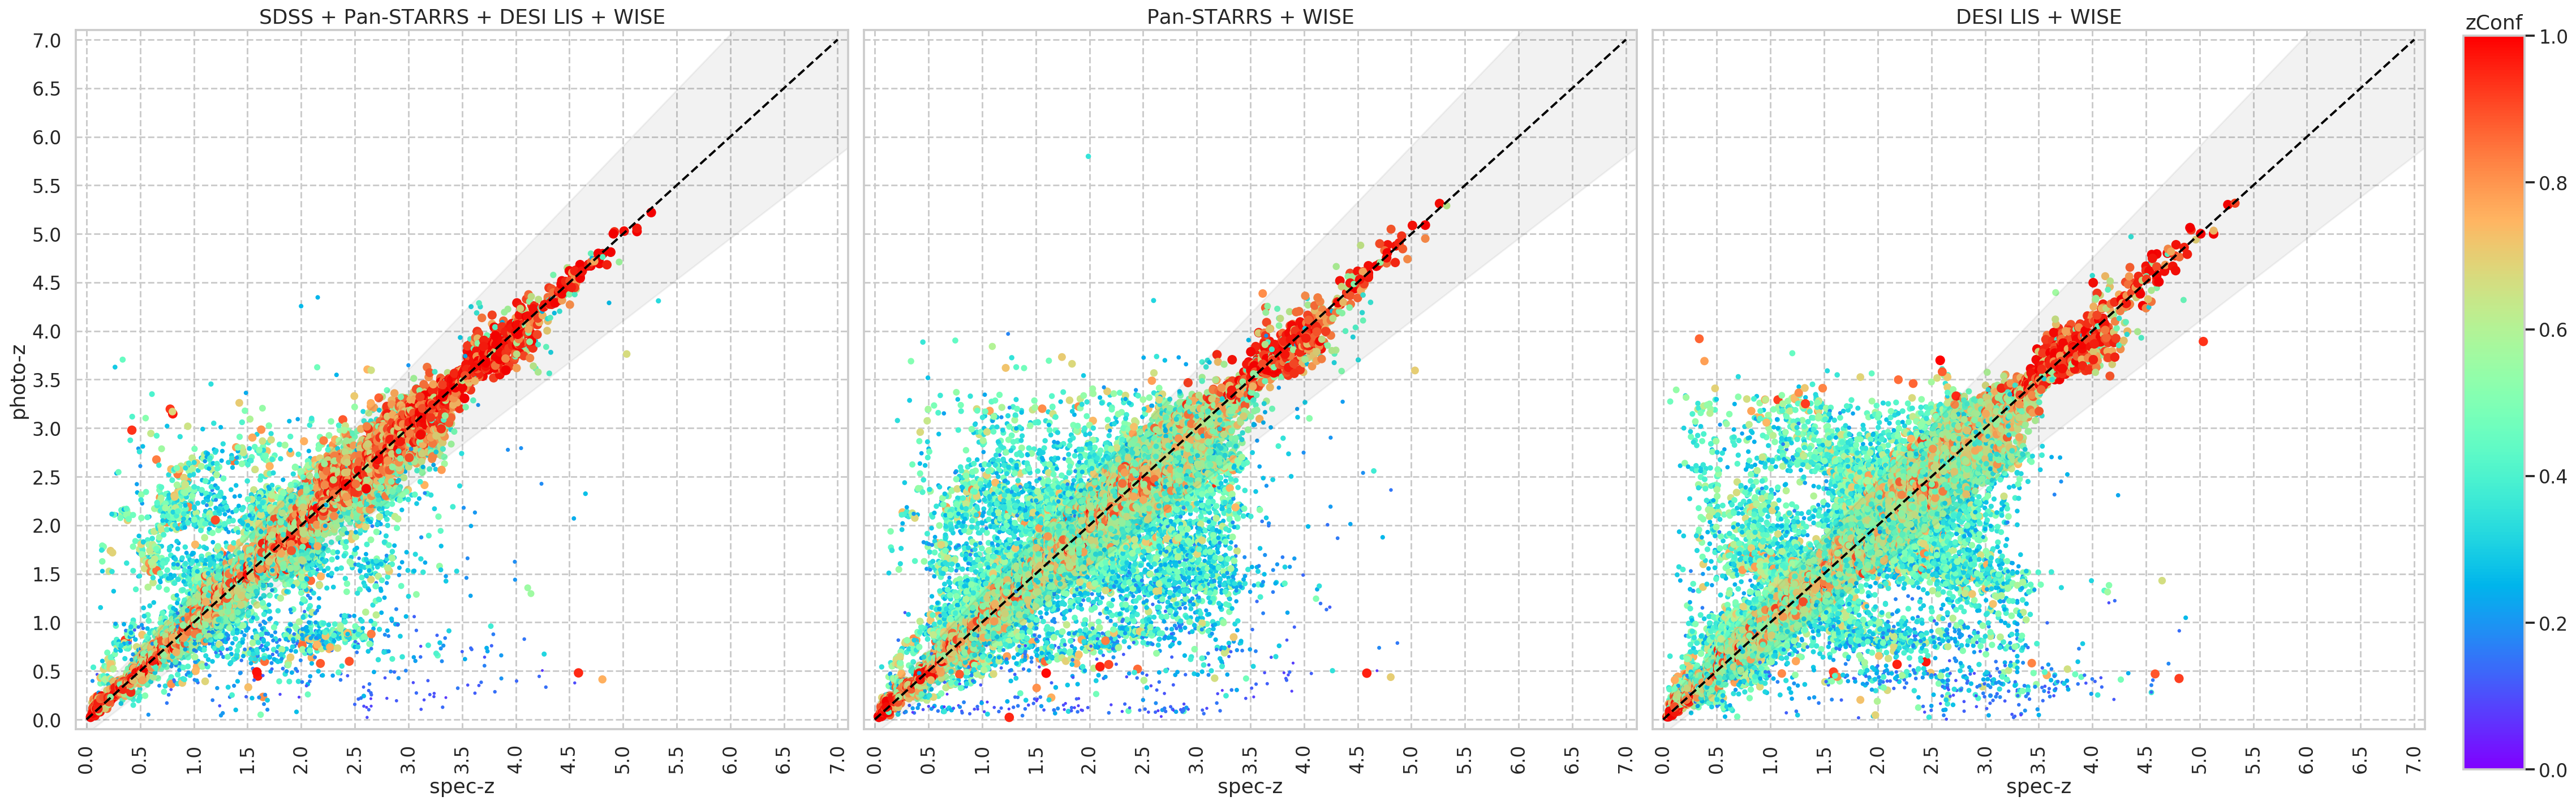
\includegraphics[width=0.9\linewidth]{images/scatterplots-dr16q-wo-train.png}
    \caption{Caption}
    \label{fig:dr16q_wo_train}
\end{figure*}

\begin{figure*}[ht]
    \centering
    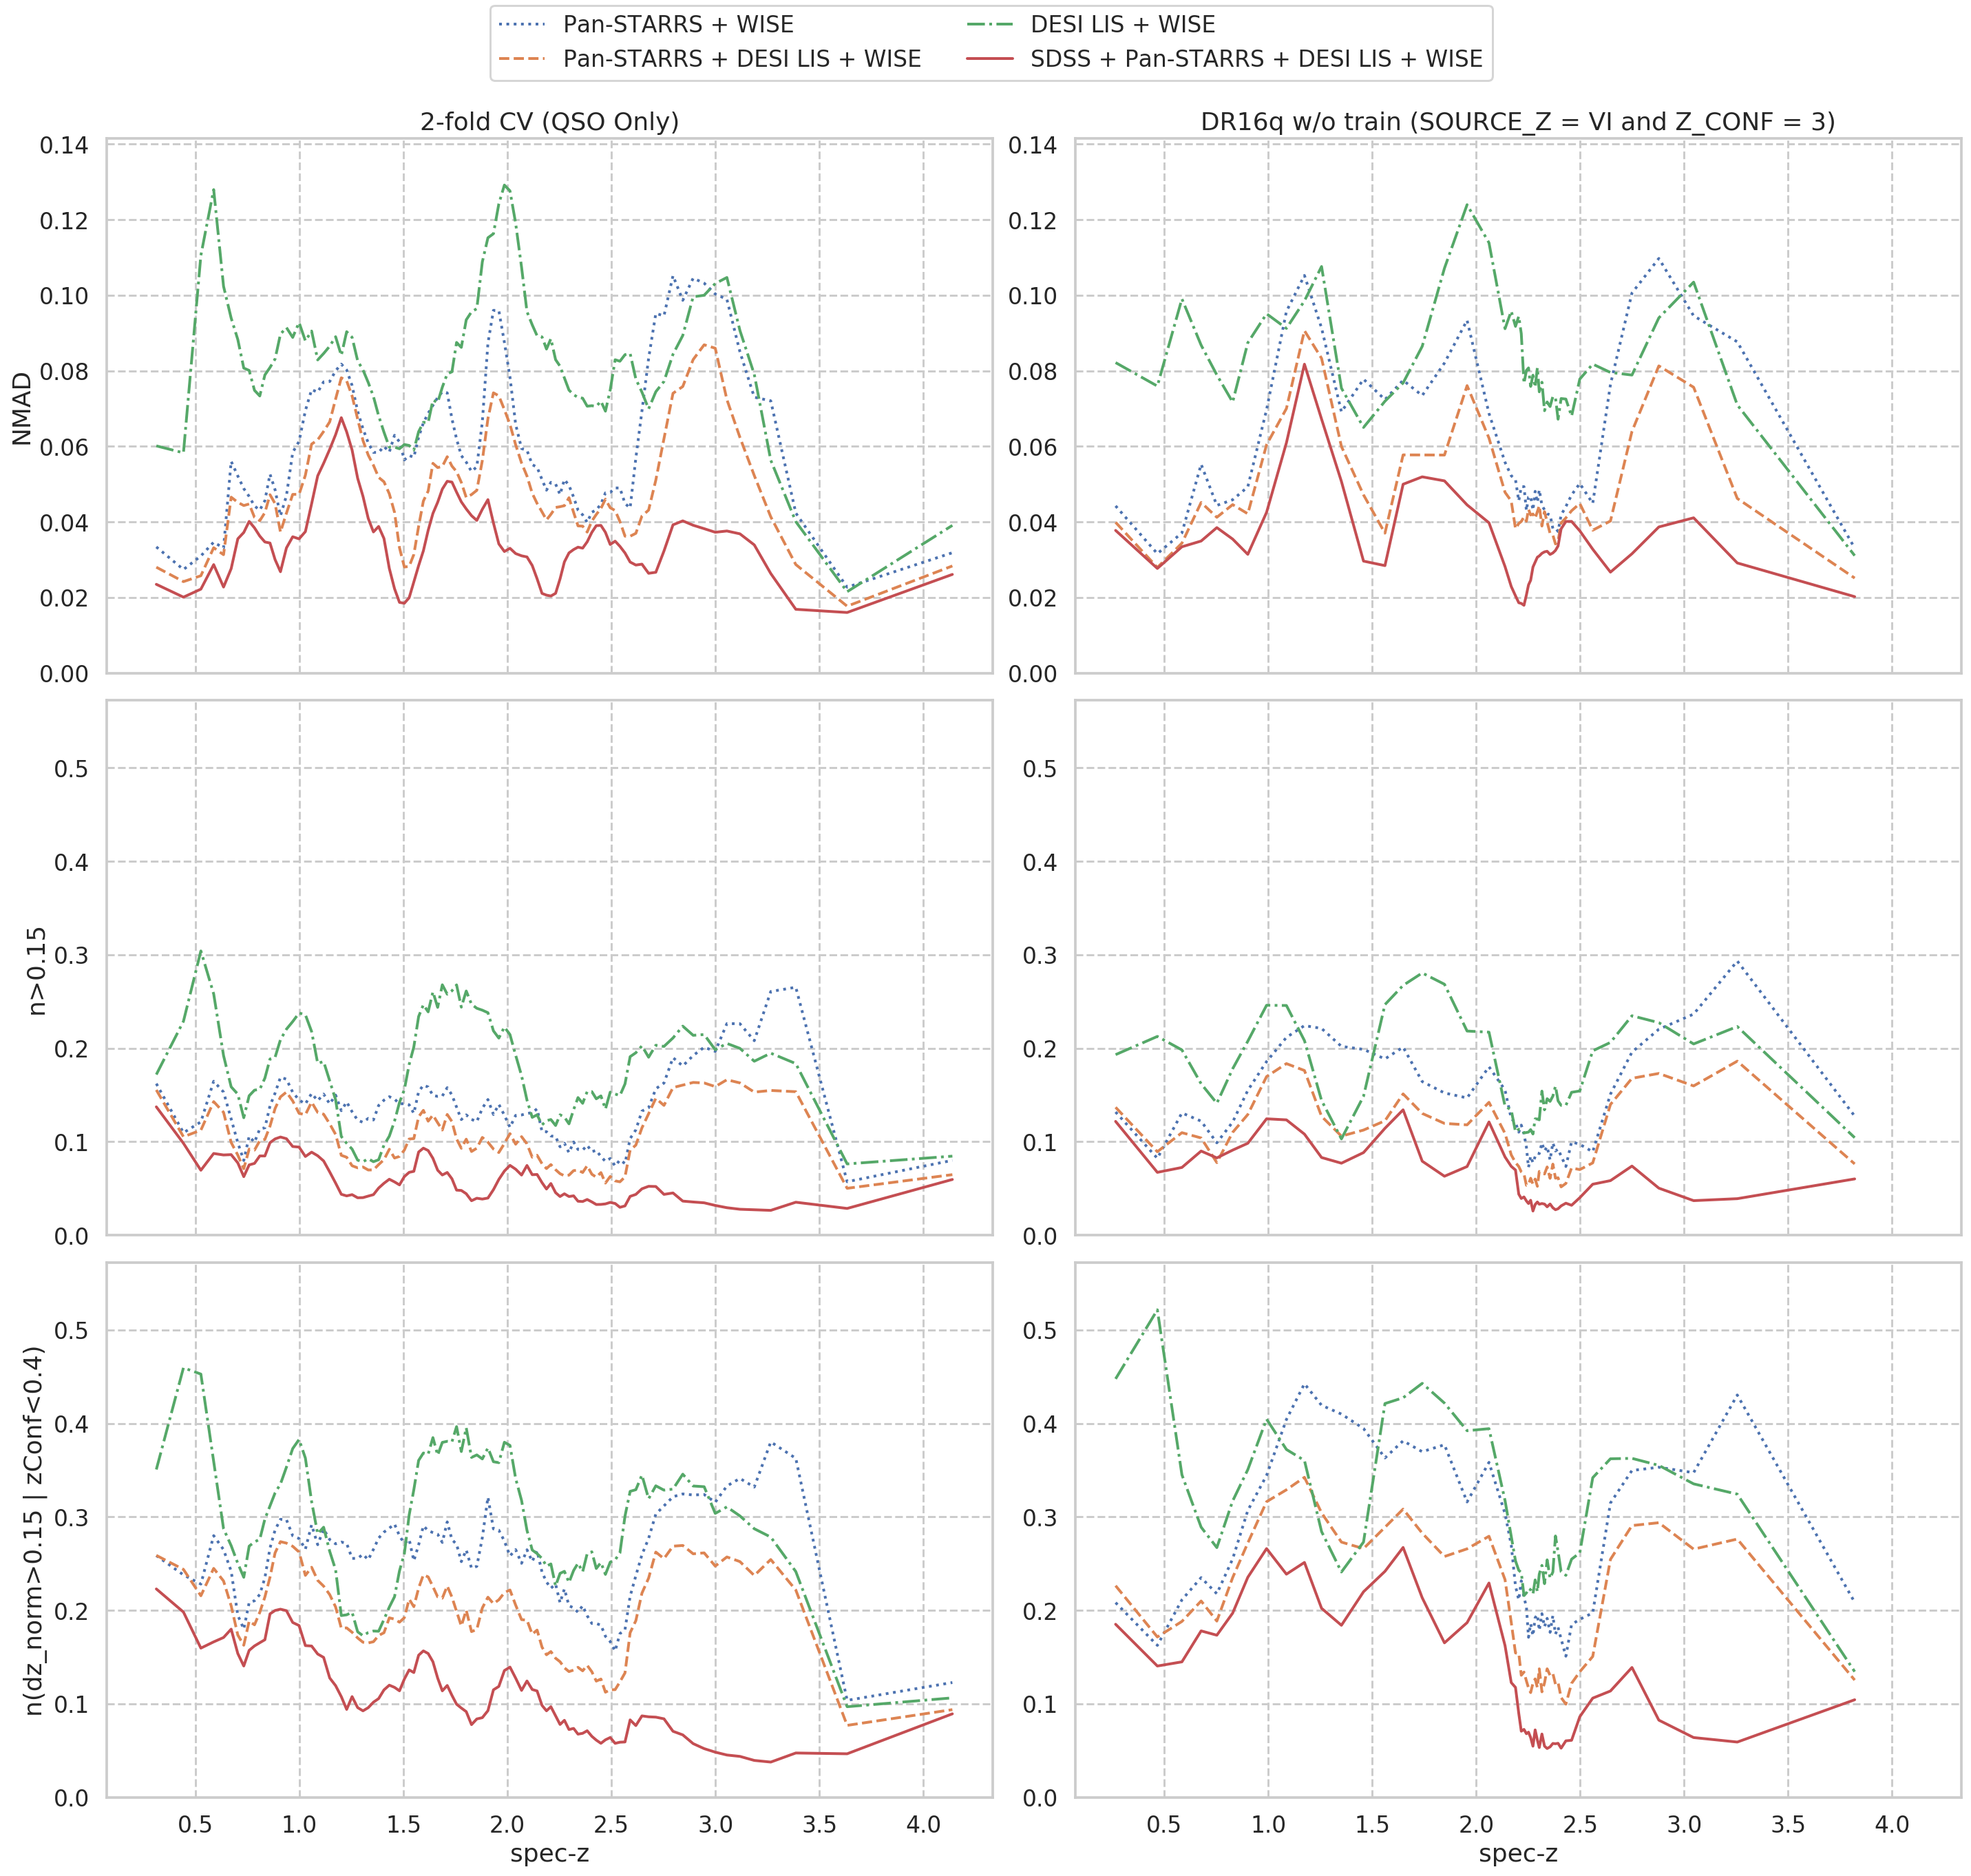
\includegraphics[width=0.9\linewidth]{images/metrics_spec-z.png}
    \caption{Caption}
    \label{fig:metrics_spec-z}
\end{figure*}

\begin{figure*}[ht]
    \centering
    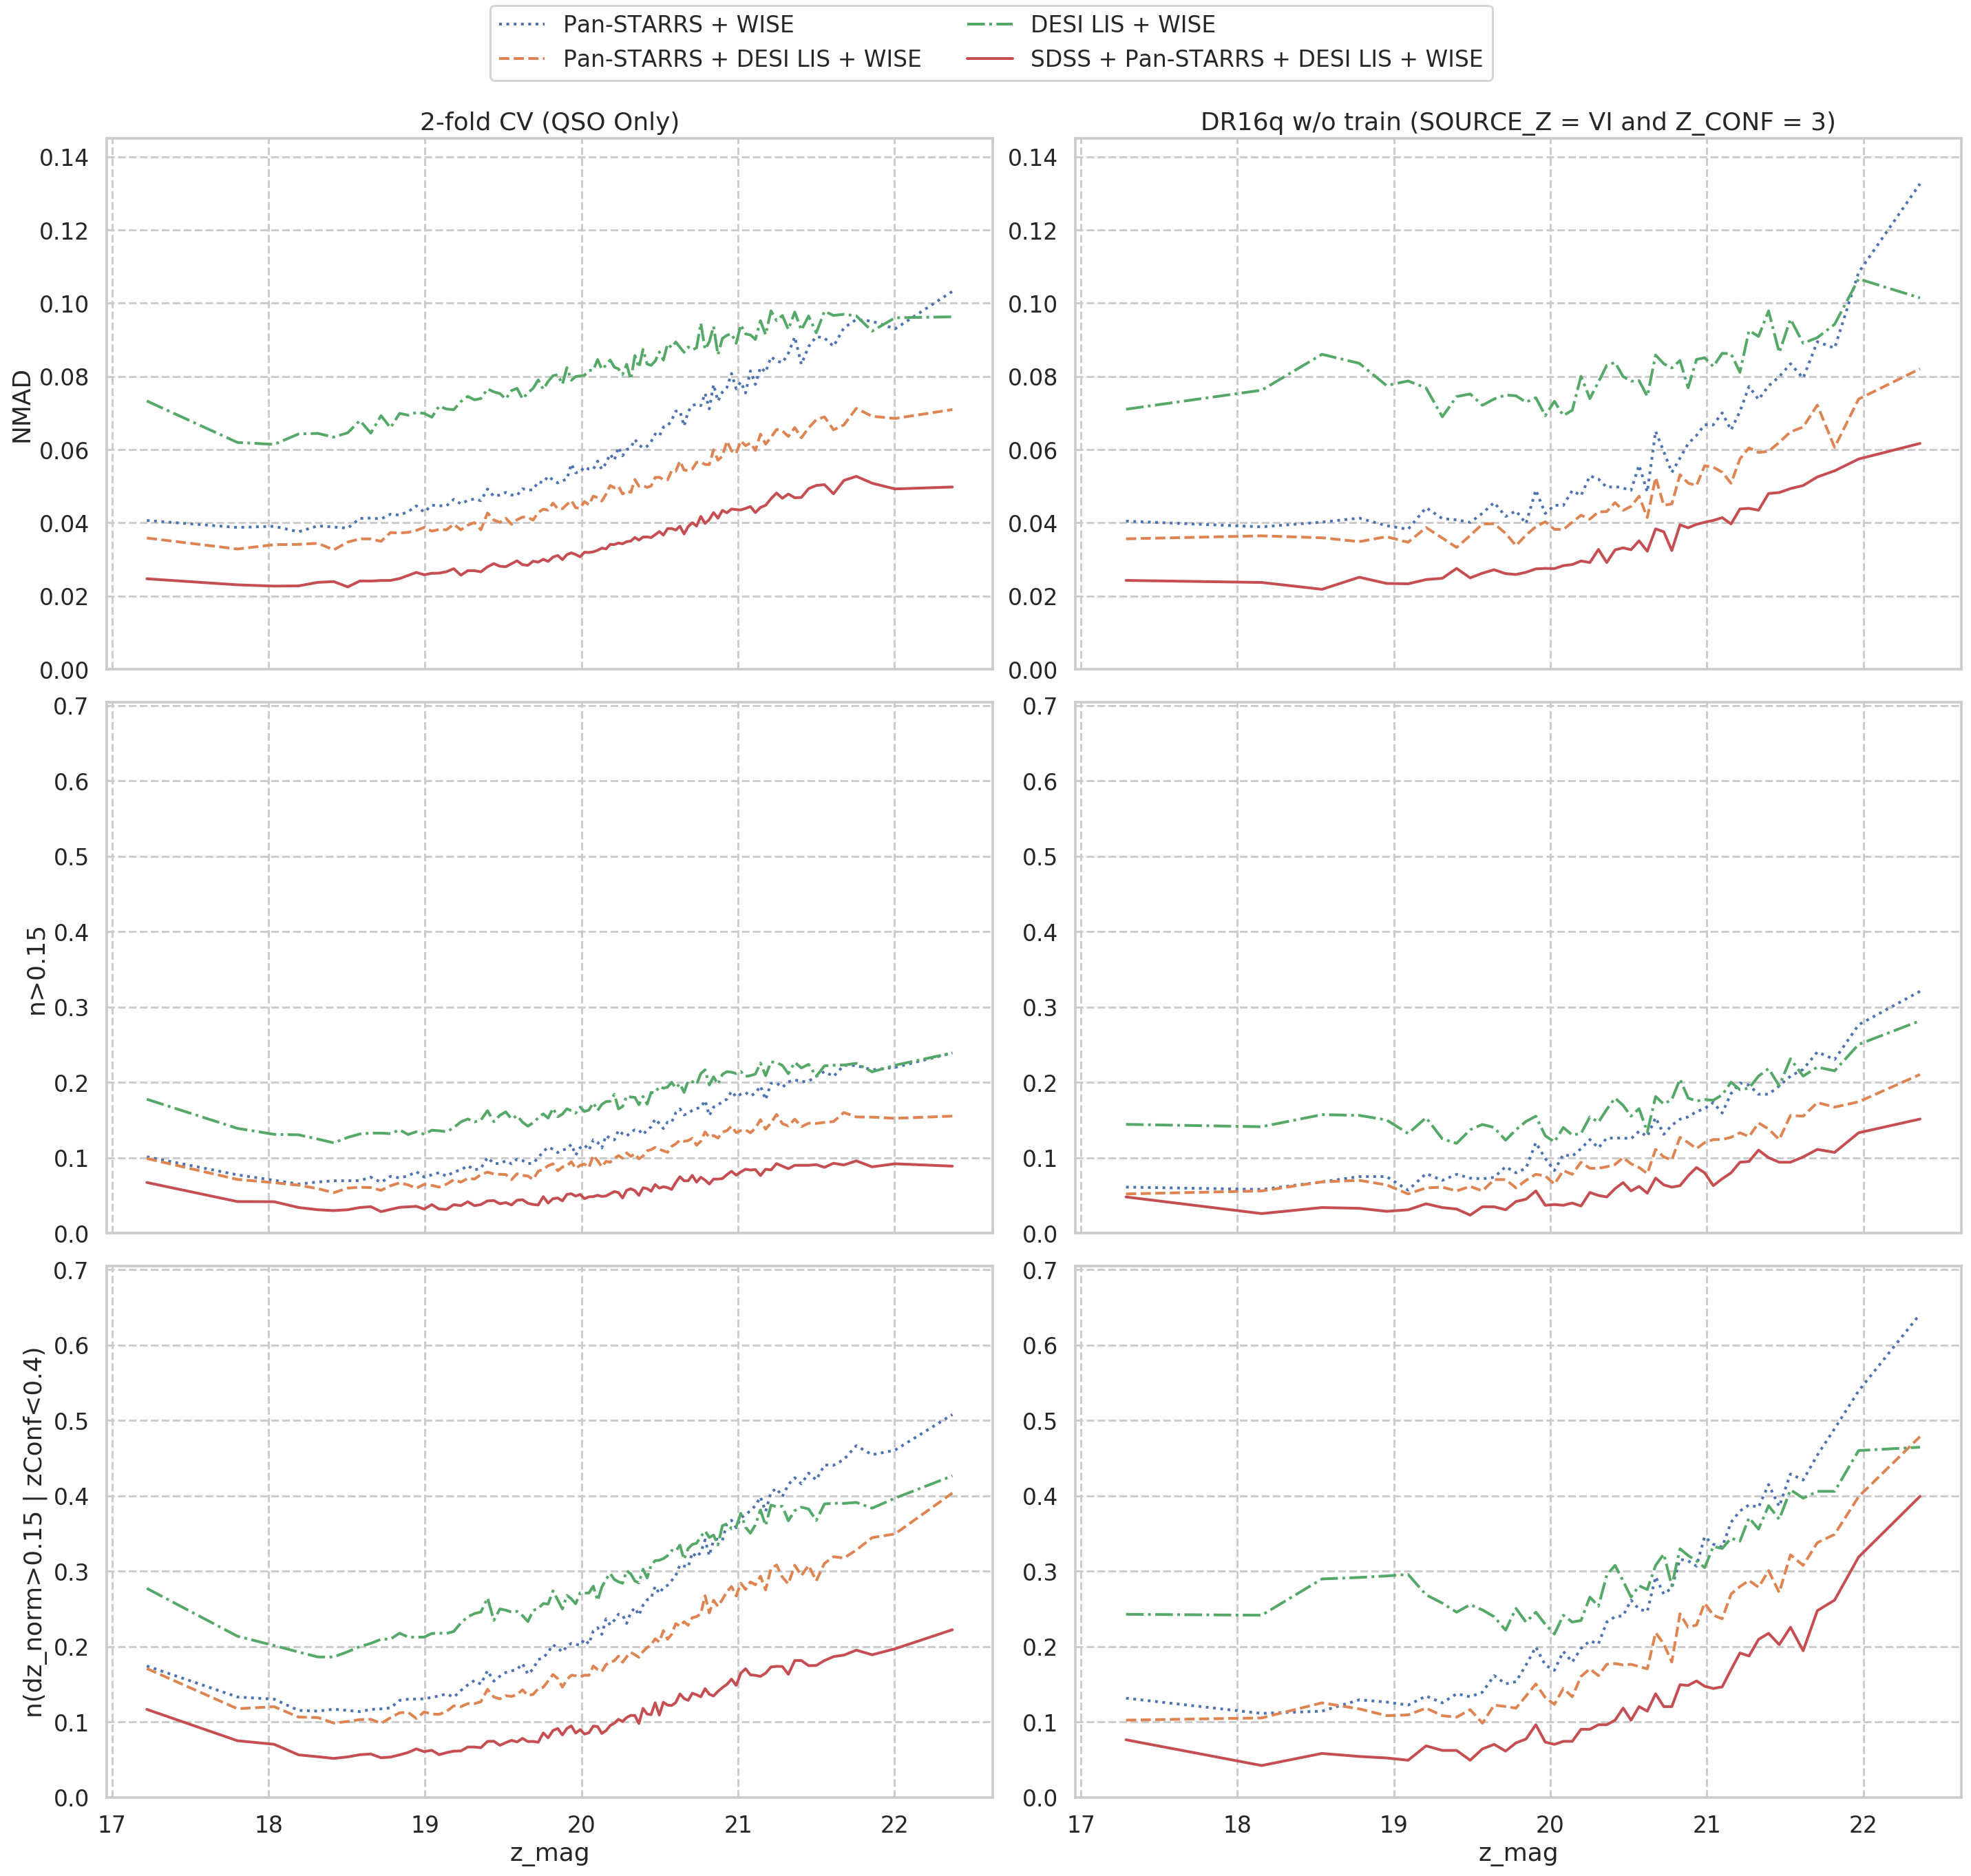
\includegraphics[width=0.9\linewidth]{images/metrics_z-mag.png}
    \caption{Caption}
    \label{fig:metrics_z_mag}
\end{figure*}

\subsection{Stripe82X results}

\begin{figure*}[ht]
    \centering
    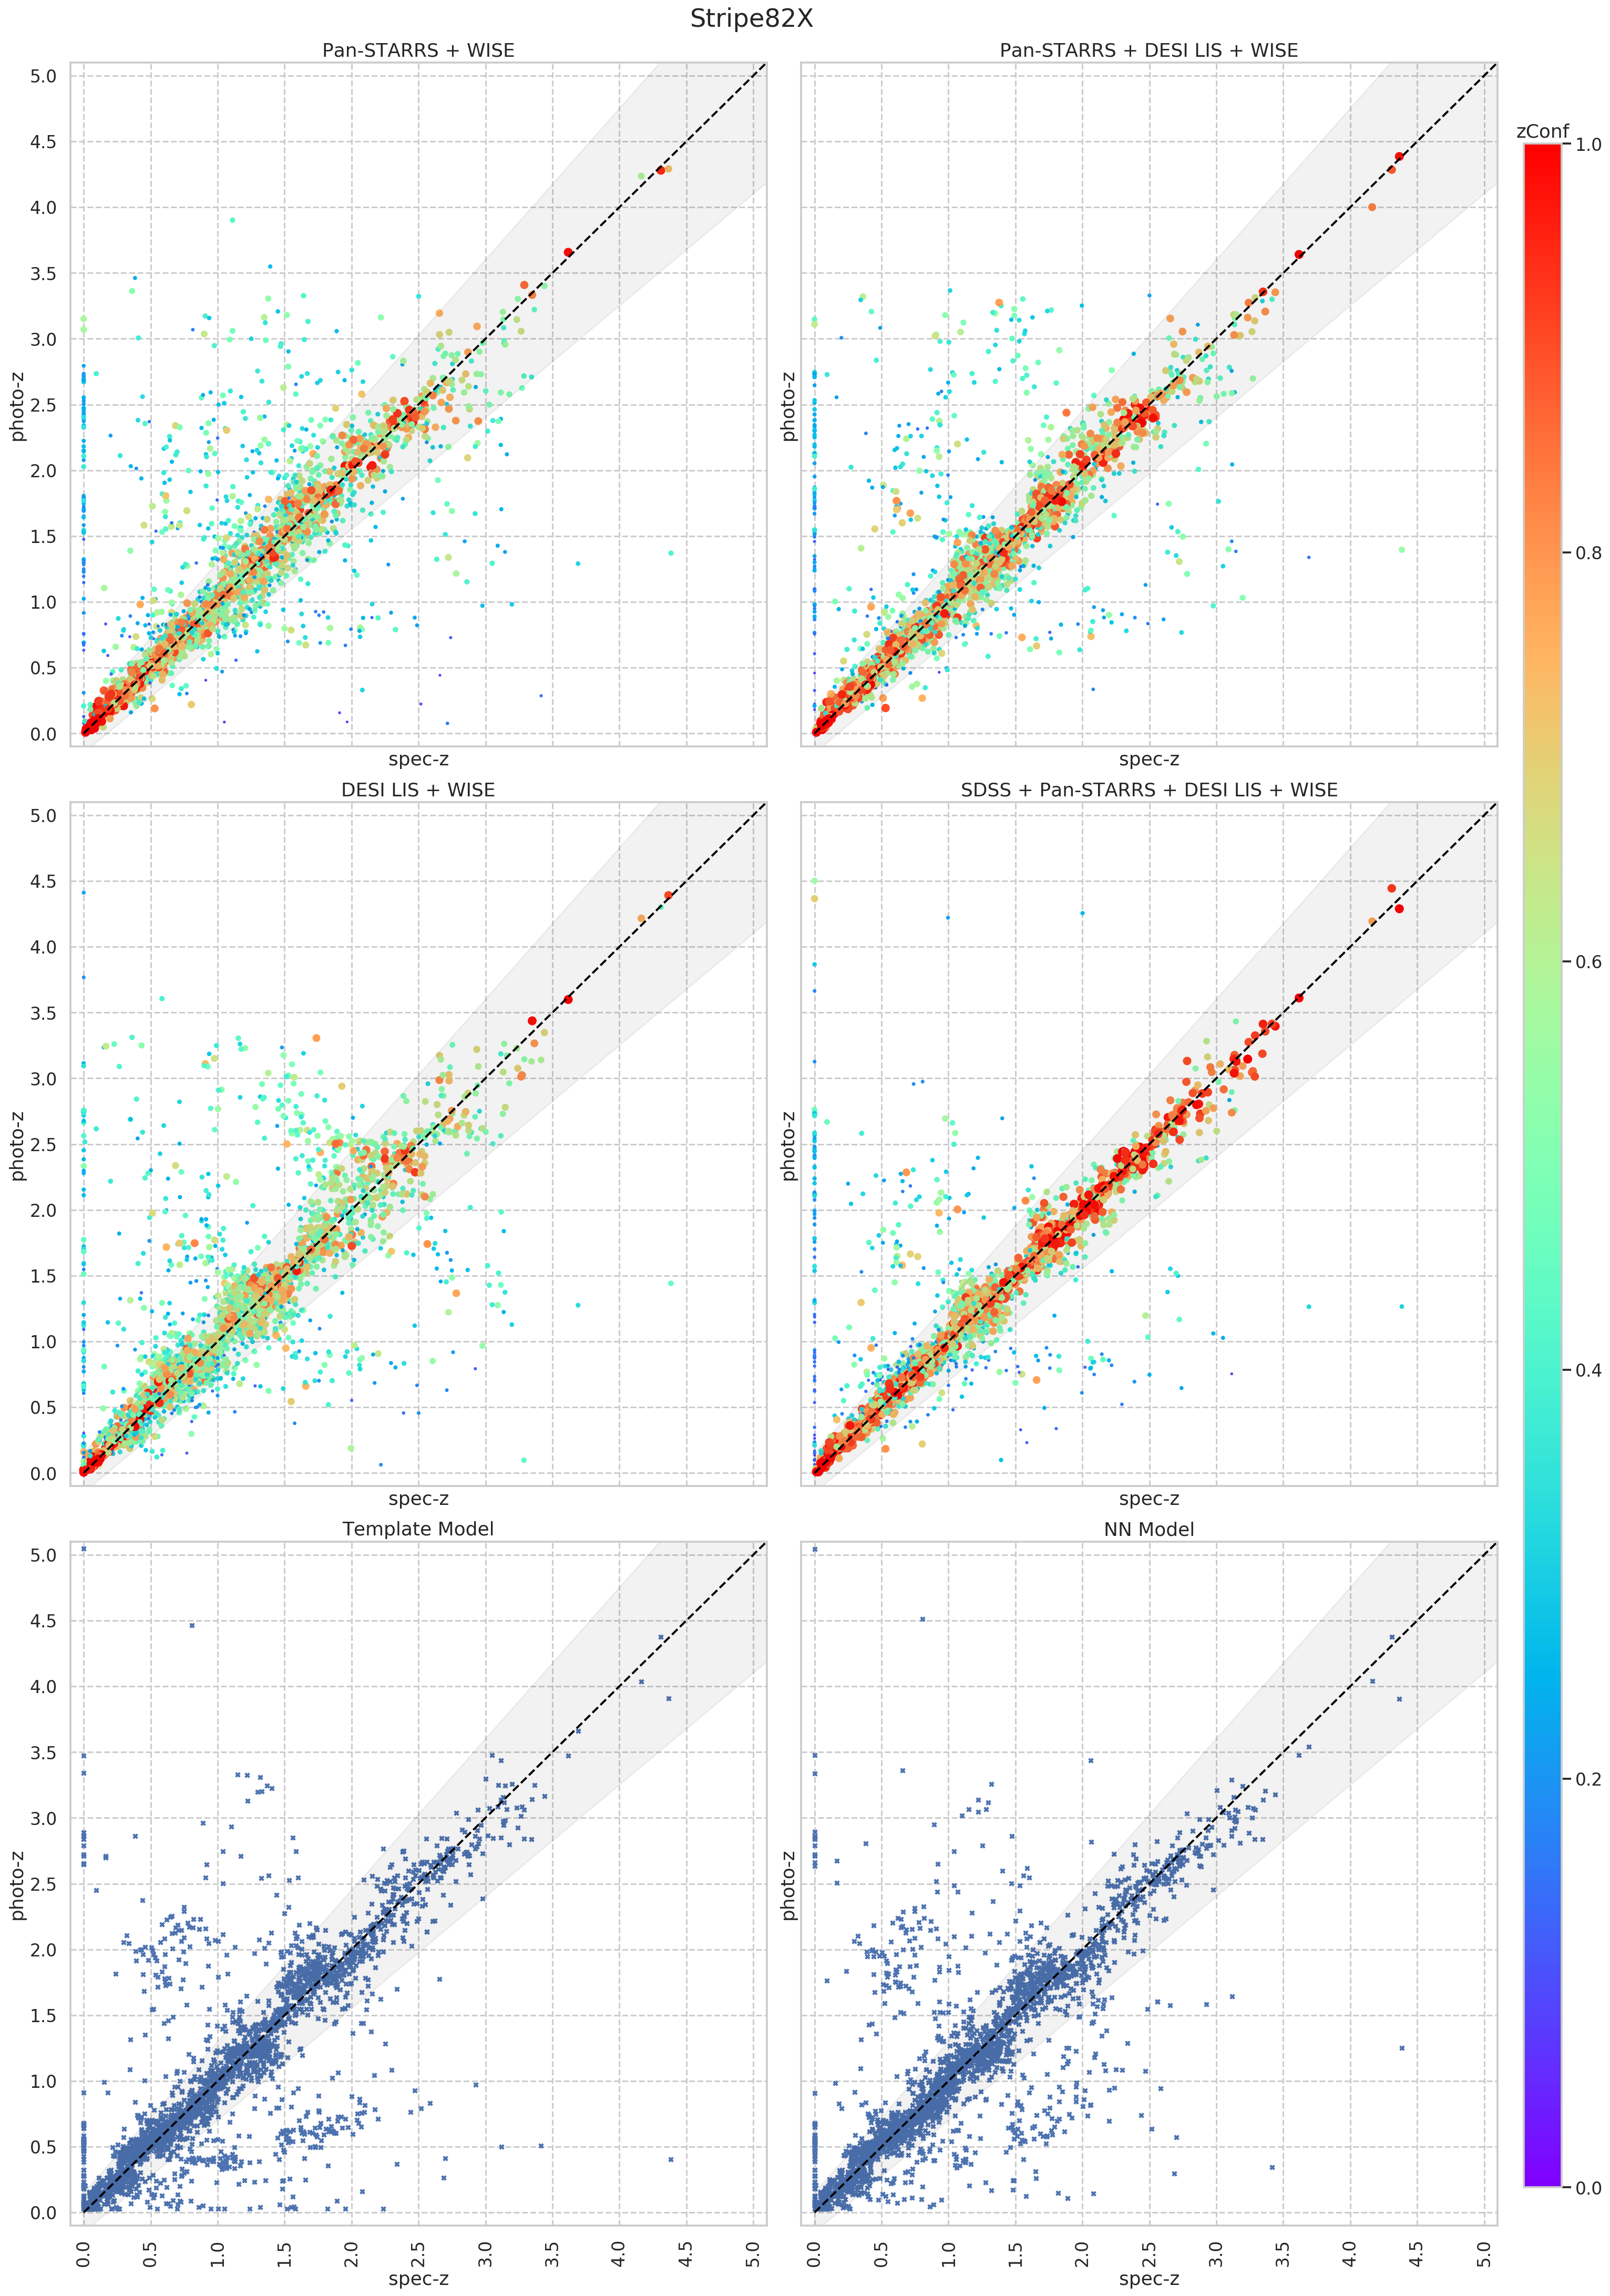
\includegraphics[width=0.9\linewidth]{images/scatterplots-stripe82x.png}
    \caption{Scatterplot on Sripe82X}
    \label{fig:s82a}
\end{figure*}

\begin{table*}
	\begin{tabular}{lccccccccc}
            \hline
            {} & \multicolumn{3}{l}{$All$ (2617 objects)} & \multicolumn{3}{l}{$z_{spec} < 0.5$ (659 objects)} & \multicolumn{3}{l}{$0.5 \leq z_{spec} < 1$ (660 objects)} \\
            {} &               $NMAD$ &        $n>0.15$ & $C_{68} - 0.68$ &                         $NMAD$ &        $n>0.15$ &  $C_{68} - 0.68$ &                                $NMAD$ &        $n>0.15$ &  $C_{68} - 0.68$ \\
            Model          &                      &                 &                 &                                &                 &                  &                                       &                 &                  \\
            \hline
            PW             &                 0.06 &           0.175 &  \textbf{0.022} &                          0.044 &           0.182 &           -0.044 &                                 0.054 &            0.15 &             0.05 \\
            PDW            &                0.048 &           0.139 &           0.054 &                          0.039 &           0.182 &           -0.032 &                                 0.047 &           0.139 &            0.067 \\
            DW             &                0.075 &           0.196 &          -0.024 &                          0.057 &           0.185 &           -0.029 &                                 0.083 &           0.211 &  \textbf{-0.025} \\
            SPDW           &       \textbf{0.036} &  \textbf{0.111} &           0.089 &                 \textbf{0.035} &  \textbf{0.175} &  \textbf{-0.008} &                        \textbf{0.038} &  \textbf{0.108} &            0.122 \\
            Template Model &                 0.07 &           0.197 &          -0.341 &                          0.085 &           0.188 &           -0.512 &                                 0.063 &            0.22 &           -0.291 \\
            NN Model       &                0.069 &           0.182 &          -0.262 &                          0.084 &           0.191 &           -0.419 &                                 0.065 &           0.198 &           -0.192 \\
            \hline
            \end{tabular}
            \caption{}
\end{table*}

\begin{table*}
	\begin{tabular}{lccccccccc}
            \hline
            {} & \multicolumn{3}{l}{$1 \leq z_{spec} < 1.5$ (546 objects)} & \multicolumn{3}{l}{$1.5 \leq z_{spec} < 2$ (402 objects)} & \multicolumn{3}{l}{$2 \leq z_{spec}$ (350 objects)} \\
            {} &                                $NMAD$ &        $n>0.15$ &  $C_{68} - 0.68$ &                                $NMAD$ &       $n>0.15$ &  $C_{68} - 0.68$ &                          $NMAD$ &        $n>0.15$ &  $C_{68} - 0.68$ \\
            Model          &                                       &                 &                  &                                       &                &                  &                                 &                 &                  \\
            \hline
            PW             &                                 0.082 &           0.196 &            0.032 &                                 0.082 &          0.167 &            0.056 &                           0.058 &           0.183 &             0.04 \\
            PDW            &                                 0.061 &           0.115 &            0.073 &                                  0.04 &          0.107 &            0.126 &                           0.048 &           0.131 &            0.083 \\
            DW             &                                 0.083 &           0.145 &  \textbf{-0.002} &                                 0.074 &          0.256 &  \textbf{-0.038} &                           0.086 &             0.2 &  \textbf{-0.031} \\
            SPDW           &                        \textbf{0.048} &  \textbf{0.088} &            0.128 &                        \textbf{0.031} &  \textbf{0.06} &            0.156 &                   \textbf{0.03} &  \textbf{0.091} &            0.071 \\
            Template Model &                                  0.07 &           0.207 &           -0.262 &                                 0.078 &          0.224 &           -0.265 &                           0.049 &           0.123 &           -0.326 \\
            NN Model       &                                 0.069 &           0.168 &           -0.189 &                                 0.067 &          0.194 &           -0.175 &                           0.053 &            0.14 &           -0.311 \\
            \hline
            \end{tabular}
            \caption{}
\end{table*}




\begin{table*}
	\begin{tabular}{lccccccccc}
            \hline
            {} & \multicolumn{3}{l}{$z_{mag} < 19$ (598 objects)} & \multicolumn{3}{l}{$19 \leq z_{mag} < 20$ (633 objects)} & \multicolumn{3}{l}{$20 \leq z_{mag} < 20.5$ (418 objects)} \\
            {} &                       $NMAD$ &        $n>0.15$ & $C_{68} - 0.68$ &                               $NMAD$ &        $n>0.15$ & $C_{68} - 0.68$ &                                 $NMAD$ &        $n>0.15$ & $C_{68} - 0.68$ \\
            Model          &                              &                 &                 &                                      &                 &                 &                                        &                 &                 \\
            \hline
            PW             &                         0.04 &           0.139 &          -0.033 &                                0.043 &           0.071 &           0.085 &                                  0.064 &           0.117 &           0.033 \\
            PDW            &                        0.033 &           0.139 &          -0.028 &                                0.036 &            0.07 &           0.111 &                                  0.046 &             0.1 &           0.107 \\
            DW             &                         0.05 &           0.156 &          -0.033 &                                0.068 &           0.118 &  \textbf{0.009} &                                  0.077 &           0.158 &  \textbf{0.014} \\
            SPDW           &               \textbf{0.027} &  \textbf{0.122} &  \textbf{0.009} &                       \textbf{0.029} &  \textbf{0.047} &           0.132 &                         \textbf{0.033} &  \textbf{0.074} &           0.109 \\
            Template Model &                        0.071 &           0.157 &          -0.548 &                                0.062 &           0.153 &          -0.396 &                                  0.064 &           0.175 &          -0.381 \\
            NN Model       &                         0.07 &           0.157 &          -0.483 &                                0.058 &           0.142 &          -0.309 &                                  0.062 &           0.151 &          -0.288 \\
            \hline
            \end{tabular}
            \caption{}
\end{table*}

\begin{table*}
	\begin{tabular}{lllllll}
            \hline
            {} & \multicolumn{3}{l}{$20.5 \leq z_{mag} < 21$ (393 objects)} & \multicolumn{3}{l}{$21 \leq z_{mag} < 23$ (572 objects)} \\
            {} &                                 $NMAD$ &        $n>0.15$ &  $C_{68} - 0.68$ &                               $NMAD$ &        $n>0.15$ &  $C_{68} - 0.68$ \\
            Model          &                                        &                 &                  &                                      &                 &                  \\
            \hline
            PW             &                                  0.064 &           0.178 &            0.038 &                                 0.12 &           0.362 &  \textbf{-0.003} \\
            PDW            &                                  0.056 &           0.137 &            0.076 &                                0.083 &           0.245 &            0.025 \\
            DW             &                                  0.088 &           0.229 &  \textbf{-0.024} &                                0.118 &           0.329 &            -0.08 \\
            SPDW           &                         \textbf{0.045} &  \textbf{0.109} &            0.106 &                       \textbf{0.065} &  \textbf{0.196} &            0.098 \\
            Template Model &                                  0.061 &           0.211 &           -0.217 &                                 0.09 &           0.294 &           -0.122 \\
            NN Model       &                                  0.063 &           0.181 &           -0.135 &                                 0.09 &           0.274 &           -0.049 \\
            \hline
            \end{tabular}
            \caption{}
\end{table*}




\begin{table*}
	\begin{tabular}{lccccccccc}
            \hline
            {} & \multicolumn{3}{l}{$FFull < 3e-15$ (2 objects)} & \multicolumn{3}{l}{$FFull < 1e-14$ (82 objects)} & \multicolumn{3}{l}{$FFull < 4e-14$ (1571 objects)} \\
            {} &                      $NMAD$ &      $n>0.15$ & $C_{68} - 0.68$ &                       $NMAD$ &       $n>0.15$ &  $C_{68} - 0.68$ &                         $NMAD$ &        $n>0.15$ & $C_{68} - 0.68$ \\
            Model          &                             &               &                 &                              &                &                  &                                &                 &                 \\
            \hline
            PW             &                        0.02 &  \textbf{0.0} &            0.32 &                        0.101 &          0.329 &           -0.119 &                          0.069 &           0.215 &  \textbf{0.006} \\
            PDW            &              \textbf{0.009} &  \textbf{0.0} &            0.32 &                        0.059 &          0.268 &           -0.034 &                          0.053 &           0.169 &           0.048 \\
            DW             &                       0.026 &  \textbf{0.0} &            0.32 &                        0.089 &           0.28 &           -0.095 &                          0.076 &           0.226 &          -0.018 \\
            SPDW           &                       0.031 &  \textbf{0.0} &            0.32 &               \textbf{0.049} &  \textbf{0.22} &  \textbf{-0.009} &                  \textbf{0.04} &  \textbf{0.137} &           0.077 \\
            Template Model &                       0.036 &  \textbf{0.0} &  \textbf{-0.18} &                        0.064 &          0.256 &           -0.326 &                          0.069 &           0.196 &            -0.3 \\
            NN Model       &                       0.034 &  \textbf{0.0} &  \textbf{-0.18} &                        0.069 &           0.28 &           -0.326 &                           0.07 &           0.183 &           -0.22 \\
            \hline
            \end{tabular}
            \caption{}
\end{table*}

\section{Conclusion}


\section{Discussion}


\section*{Acknowledgments}
..

% bibliograpgy 
\bibliographystyle{mnras}
\bibliography{main}

\appendix

\section{..}

\end{document}
